\documentclass[12pt,a4paper]{report}
\usepackage[utf8]{inputenc}
\usepackage{graphicx}
\usepackage{hyperref}
\usepackage{setspace}
\usepackage{geometry}
\geometry{left=3cm,right=2.5cm,top=3cm,bottom=3cm}

\setlength{\parskip}{1em}
\setlength{\parindent}{0pt}
\onehalfspacing

% Title and author info
\title{Your Seminar Report Title}
\author{Your Name \\ Department of XYZ \\ Your College Name}
\date{\today}

\begin{document}
	\begin{titlepage}
	\centering
	\vspace*{3cm}
	{\Huge \bfseries JSONPath \par}
	{\Large \textbf{Structure, Parsing, and Applications in Data Analytics and NLP} \par}
	\vspace{2cm}
	{\Large by \par}
	\vspace{0.5cm}
	{\Large \textbf{Goti, Jenil Jagdishbhai} \par}		
	\vspace{0.5cm}
	{\large Supervised by \par}
	{\Large \textbf{Prof. Bantel, Winfried} \par} 
	\vfill
	{\large Department of Elektronik und Informatik \par}
	{\large \textbf{Hochschule Aalen – Technik, Wirtschaft und Gesundheit} \par}
	{\large \today \par}
\end{titlepage}

	\chapter*{Abstract}
This report is about JSONPath, which is used to retrieve data from JSON object. Nowadays,it is used everywhere. In this report, I explain previous researches abut it, how JSONPath works, what is its structure and how to build a parser that understands these expressions. I also explains about where JSONPath is useful, especially in data analysis and natural language processing, helping us to understand messy or nested data. Overall, this report gives a clear look at how JSONPath can be used to make handling JSON simpler and more effective.

	\newpage
	\tableofcontents
	\newpage
	\chapter{Introduction}

JavaScript Object Notation (JSON) is a lightweight, text-based data interchange format widely used for communication between web clients and servers. Its simplicity, readability, and ability of parsing have made it very impotent in today's software systems for exchanging structured data.

Parsing JSON data efficiently and accurately is critical to ensure seamless data transfer and integration between heterogeneous systems. A JSON parser reads JSON text, check its correct or not according to the JSON syntax, and converts it into valid data structures for a program. This process is being an essential part of many applications, web APIs, configuration management, and real-time data processing.

The key goal behind this seminar report is to research about the design and implementation of a JSON parser, understand the parsing techniques, and evaluate parser performance. By developing a custom JSON parser, this report aims to provide knowledge into compiler construction concepts such as lexical analysis, syntax parsing, and error handling relevant to a practical and widely used data format.

The objectives of this seminar report are as follows:
\begin{itemize}
	\item To study the JSON format, its syntax, and grammar rules.
	\item To analyze different parsing techniques applicable for JSON, including recursive descent and LR parsing.
	\item To implement a JSON parser using tools like Lex and Yacc, focusing on accurate parsing and error detection.
\end{itemize}

This report based on the syntax parsing aspects of JSON, error handling mechanisms, and practical implementation details. 

The report is organized as following: Chapter 2 have details existing JSON parsers and parsing techniques. Chapter 4 is about the methodology used for the parser design and implementation. Chapter 5 gives the results, testing, and analysis of the parser. Finally, Chapter 5 is the conclusion  the report and suggests directions for future enhancements.

With this seminar report, readers can understand a comprehensive understanding of JSON parsing and get practical knowledge to compiler construction techniques applied to a real-world problem.

	\chapter{Literature Survey}

\section{Overview of JSON and JSON Parsing}

JavaScript Object Notation (JSON) is a lightweight, text-based data format mainly used for data transfer in modern applications. It shows data using key-value pairs, arrays, and nested objects, developing it both human-readable and easy for machines to parse~\cite{ietf_rfc9535}.

JSON is mainly used in REST APIs, configuration of files, and client-server communication. Efficient parsing of JSON is impotent for the performance and reliability of software systems~\cite{sql_json_wiscorp}.

A JSON parser reads JSON text and transfer it into internal data structures like dictionaries or arrays. Parsers strictly follow the JSON syntax defined in RFC 8259 to ensure that it is correct or not and interoperability~\cite{ietf_rfc9535}.

\section{Existing JSON Parsers}

Many JSON parsers exist for many programming languages, works for both basic parsing and advanced querying features such as JSONPath:

\begin{itemize}
	\item \textbf{Built-in parsers}: Many languages include native JSON parsing, such as \texttt{JSON.parse()} in JavaScript, \texttt{json.loads()} in Python, and Java’s \texttt{JSON.parse()}~\cite{programmerall_article}.
	\item \textbf{Database parsers}: Modern databases like PostgreSQL support JSON and JSONB data types and gives built-in JSONPath query parsing and execution capabilities~\cite{postgres_jsonpath}.
	\item \textbf{Library-based parsers}: Libraries like JsonCons.Net for C\# and Jackson for Java offer rich JSON parsing and JSONPath querying support~\cite{jsoncons_net}.
	\item \textbf{Node.js JSONPath libraries}: In JavaScript server environments, libraries like \texttt{jsonpath} by Bruno Sciessere (brunerd/jsonpath) gives flexible and powerful JSONPath querying functionality~\cite{brunerd_jsonpath}. These makes complex JSONPath expressions to be evaluated efficiently in Node.js applications.
	\item \textbf{Custom and grammar-based parsers}: Tools like ANTLR4 gives grammar specifications to develop parsers capable of processing JSON and JSONPath queries~\cite{antlr4_jsonpath}.
\end{itemize}

These parsers differ in performance, feature completeness, and error-handling.

\section{Parsing Techniques}

Parsing JSON typically involves two key stages:

\begin{enumerate}
	\item \textbf{Lexical Analysis (Tokenization)}: separate input JSON text into tokens like strings, numbers, brackets, and punctuation.
	\item \textbf{Syntactic Analysis (Parsing)}: compare tokens with grammar rules to generate data structures.
\end{enumerate}

Common parsing technics:

\begin{itemize}
	\item \textbf{Recursive Descent Parsing}: it is a top-down method and parsing functions call themselves to handle nested data structures. Applicable for JSON’s with simple grammar~\cite{jsonpath_plus}.
	\item \textbf{LR Parsing}: it is a bottom-up parsing approach for parser generators like Bison or Yacc, which reduce input tokens with grammar rules to build parse trees~\cite{postgres_jsonpath}.
	\item \textbf{Parsing Expression Grammars (PEG)}: Available in some modern parsers for their expressive power and User-friendliness. ~\cite{antlr4_jsonpath}.
\end{itemize}

JSONPath parsers use these techniques to handle expressions like filters, wildcards, recursive descent selectors, and array slicing, requiring enhanced grammar and evaluation logic~\cite{ietf_rfc9535}.

\section{Challenges in JSON Parsing}

\begin{itemize}
	\item \textbf{Handling Deep Nesting}: It is possible that JSON objects and arrays is deeply nested and it is require for parsers to accurately manage recursion and memory consumption~\cite{toolsqa_jsonpath}.
	\item \textbf{Error Detection and Recovery}: Parsers need to detect malformed JSON or invalid JSONPath expressions and recover where possible~\cite{jsonpath_com}.
	\item \textbf{Performance}: Large JSON documents and complex queries need parsers optimization for speed and low memory consumption~\cite{programmerall_article}.
	\item \textbf{Supporting Advanced Query Features}: developing complex filters, logical expressions, array slicing, and recursive descent in JSONPath requires a high degree of complexity for grammar design and evaluation strategies~\cite{ietf_jsonpath_draft}.
	\item \textbf{Standards Compliance}: Parsers need to act according to formal specifications like RFC 8259 (JSON) and RFC 9535 (JSONPath) to make sure interoperability across systems~\cite{ietf_rfc9535,ietf_jsonpath_draft}.
\end{itemize}

\section{Summary}

In summary, JSON is a basic data format which need complex and affective parsing solutions. There is many parsers starting from simple language built-ins to advanced libraries and database engines supporting complex JSONPath querying~\cite{brunerd_jsonpath,jsoncons_net,postgres_jsonpath}.

Parsing methods like recursive descent and LR parsing gives the foundation for reliable JSON and JSONPath processing. However, challenges like deep nesting, error handling, performance, and supporting complex queries still remain important~\cite{toolsqa_jsonpath}.

To understand existing parsers, their techniques, and the available challenges gives deep understanding for designing efficient and robust JSON and JSONPath parsers.

	\chapter{Grammar, Syntax, and Examples of JSONPath}

\section{Formal Grammar}

JSONPath expressions are based on a formal grammar that provide the syntax rules for querying JSON data. The grammar make sure that JSONPath expressions are parsable by JSON parsers.  
A simple version of the JSONPath grammar, inspired by the IETF drafts \cite{ietf_jsonpath_draft, ietf_rfc9535} and implementations like PostgreSQL’s \texttt{jsonpath\_gram.y} \cite{postgres_jsonpath}, is given below using a Backus-Naur Form (BNF)-style notation:

\begin{quote}
	\begin{tabbing}
		jsonpath       ::= root-selector selector-list \\
		root-selector  ::= '\$' 
		selector-list  ::= selector selector-list \textbar\ $\epsilon$ \\
		selector       ::= '.' child-name \\
		\quad \textbar\ '..' recursive-name \\
		\quad \textbar\ '[' array-index ']' \\
		\quad \textbar\ '[' array-slice ']' \\
		\quad \textbar\ '[' filter ']' \\
		child-name     ::= NAME \\
		recursive-name ::= NAME \\
		array-index    ::= INTEGER \\
		array-slice    ::= INTEGER? ':' INTEGER? (':' INTEGER?)? \\
		filter         ::= '?(' expression ')' \\
		expression     ::= \dots
	\end{tabbing}
\end{quote}

Here:  
- \texttt{\$} is the root object of the JSON.  
- \texttt{@} is the current node in filter expressions.  
- Selectors allow navigation to child elements, recursive descent, array elements, or filtered subsets.

\section{Core Syntax and Expressions}

The primary syntax components of JSONPath are available in the IETF JSONPath standard \cite{ietf_rfc9535} and popular tutorials \cite{toolsqa_jsonpath, azure_jsonpath}:

\begin{itemize}
	\item \textbf{Root Selector (\$)}: the root of the JSON data.
	\item \textbf{Current Node (@)}: the current context node, primarily used in filter expressions.
	\item \textbf{Dot Notation (.)}: Selects child members by name, e.g., \texttt{.store}.
	\item \textbf{Recursive Descent (..)}: Searches recursively for matching child elements at any depth.
	\item \textbf{Wildcards (*)}: Matches all elements in an array or all keys in an object.
	\item \textbf{Array Indexing and Slicing}:  
	- Single index: \texttt{[0]}, \texttt{[1]} selects elements by position.  
	- Slice: \texttt{[start:end:step]} selects a range of elements.
	\item \textbf{Filters ([?()])}: Allows selection based on expressions, such as comparisons or logical operations inside brackets.  
	\item \textbf{Expressions inside Filters}:  
	- Comparison operators: \texttt{==, !=, <, >, <=, >=}  
	- Logical operators: \texttt{\&\& (and), || (or), ! (not)}  
	- Functions: \texttt{length()}, \texttt{sum()}, etc.
\end{itemize}

\section{Examples}

The following JSON data represent a bookstore \cite{toolsqa_jsonpath}:

\begin{verbatim}
	{
		"store": {
			"book": [
			{
				"category": "reference",
				"author": "Nigel Rees",
				"title": "Sayings of the Century",
				"price": 8.95
			},
			{
				"category": "fiction",
				"author": "Evelyn Waugh",
				"title": "Sword of Honour",
				"price": 12.99
			},
			{
				"category": "fiction",
				"author": "Herman Melville",
				"title": "Moby Dick",
				"price": 8.99
			}
			],
			"bicycle": {
				"color": "red",
				"price": 19.95
			}
		}
	}
\end{verbatim}

Some JSONPath queries and their explanations:

\begin{itemize}
	\item \texttt{\$.store.book[*].author}  
	Selects the authors of all books in the store.  
	\textbf{Result:} \texttt{["Nigel Rees", "Evelyn Waugh", "Herman Melville"]}
	
	\item \texttt{\$.store.book[0]}  
	Selects the first book in the array.  
	\textbf{Result:} The entire JSON object for the first book.
	
	\item \texttt{\$.store.book[?(@.price < 10)].title}  
	Selects titles of books with a price less than 10.  
	\textbf{Result:} \texttt{["Sayings of the Century", "Moby Dick"]}
	
	\item \texttt{\$.store..price}  
	Recursively selects all prices in the store (books and bicycle).  
	\textbf{Result:} \texttt{[8.95, 12.99, 8.99, 19.95]}
	
	\item \texttt{\$..author}  
	Selects all authors in the document regardless of depth.  
	\textbf{Result:} \texttt{["Nigel Rees", "Evelyn Waugh", "Herman Melville"]}
\end{itemize}

These examples shows how JSONPath expressions gives powerful and flexible ways to navigate and extract data from complex JSON structures.

	\chapter{Methodology}

\section{Overview}

In this section, we can see the details of the approach taken to design and implement the JSONPath parser. It includes the system architecture, parsing techniques, grammar design, implementation details, error handling strategies, and testing methodology.

\section{System Architecture}

The JSONPath parser system is built with some many key components:

\begin{itemize}
	\item \textbf{Lexer (Tokenizer)}: Converts the input JSONPath query string into a stream of tokens like identifiers, operators, brackets, and literals.
	\item \textbf{Parser}: Processes the token stream according to the JSONPath grammar to build a parse tree representing the query structure.
	\item \textbf{Evaluator}: Traverses the parse tree to evaluate the query against input JSON data, retrieving the requested nodes or values.
	\item \textbf{Error Handler}: Find out and reports syntax errors in the JSONPath expressions, giving meaningful feedback to the user.
\end{itemize}

\section{Parsing Approach}

The parser is developed using a \textbf{recursive descent parsing} technique due to JSONPath’s relatively straightforward and context-free grammar. This approach used for clear, modular parsing functions for each grammar rule, making the parser easier to maintain and extend.

Moreover, parser generators such as Bison and Flex could be used to implement an LR parser; however, recursive descent was chosen for its simplicity and flexibility in handling filters and expressions within JSONPath.

\section{Grammar Design}

The grammar of JSONPath was adapted from the IETF JSONPath specification (RFC 9535) and existing implementations such as PostgreSQL’s \texttt{jsonpath\_gram.y}. Impotent grammar rules are following:

\begin{itemize}
	\item \textbf{Root Selector}: The starting point symbol \texttt{\$}.
	\item \textbf{Child and Recursive Descent}: Operators \texttt{.} and \texttt{..} select child nodes or recursively descend into nested structures.
	\item \textbf{Array Indexing and Slicing}: Square brackets \texttt{[ ]} used to select array elements by index or slices.
	\item \textbf{Filters}: Expressions inside \texttt{[?()]} gives conditional selection according on logical and comparison operators.
\end{itemize}

The grammar was built in a modular manner, with separate parsing functions handling selectors, filters, expressions, and literals.

\section{Implementation Details}

The parser is developed with \textbf{C++} (or specify your language) using modern programming. necessary tools and libraries include:

\begin{itemize}
	\item \textbf{Lexer}: A hand-written tokenizer that reads input character-by-character to generate tokens.
	\item \textbf{Parser}: Recursive descent functions developed manually without parser generator tools.
	\item \textbf{JSON Library}: make practical and effective use of a third-party JSON library such as \texttt{nlohmann/json} for parsing and manipulating input JSON data.
	\item \textbf{Development Environment}: Built and tested using \texttt{g++} compiler on Linux, with \texttt{CMake} for build automation.
\end{itemize}
\begin{figure}[htbp]
	\centering
	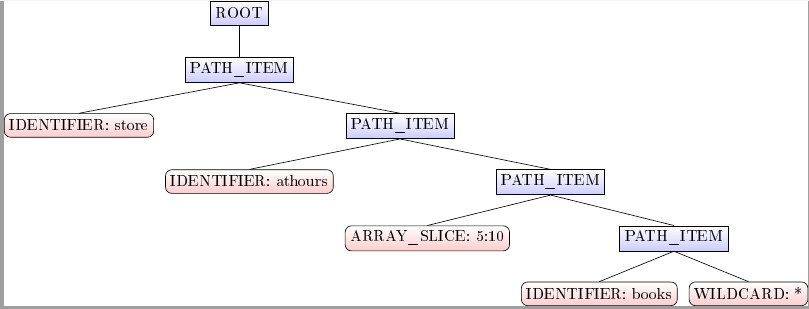
\includegraphics[width=0.7\textwidth]{images/op_graph.png}
	\caption{Sample output of the JSONPath parser evaluating a query on test JSON data.}
	\label{fig:parser_output}
\end{figure}

\section{Integration with YottaDB Query}

To add the functionality in the JSONPath parser, the parsed queries are compiled into YottaDB query language statements. This gives seamless querying of JSON-like hierarchical data stored in the YottaDB database.

The compilation process converts JSONPath expressions such as property selectors, filters, and array indexing into equivalent YottaDB query commands, allow execution of query within the database environment.

Figure~\ref{fig:yottadb_output} shows a sample output of a compiled JSONPath query executed on YottaDB data.

\begin{figure}[htbp]
	\centering
	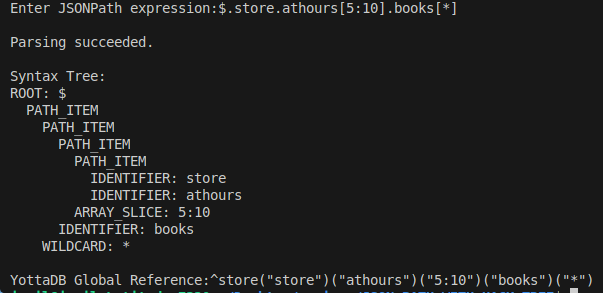
\includegraphics[width=0.7\textwidth]{images/yottadb_output.png}
	\caption{Output of the JSONPath query compiled and executed as a YottaDB query.}
	\label{fig:yottadb_output}
\end{figure}

\section{Error Handling}

The parser includes error detection to handle:

\begin{itemize}
	\item \textbf{Syntax Errors}: Missing brackets, invalid tokens, or unexpected symbols in JSONPath expressions are reported with descriptive error messages.
	\item \textbf{Semantic Errors}: Wrong filter expressions or unsupported operations gives errors.
\end{itemize}

Error handling allows the parser to terminate when it needed or used for limited recovery where possible, improving user experience.

\section{Testing and Validation}

To make sure parser is correct and robust or not, it was tested using:

\begin{itemize}
	\item \textbf{Unit Tests}: Cover individual parser functions and lexer components, including edge cases.
	\item \textbf{Test JSON Datasets}: Sample JSON documents representing various complexities and structures.
	\item \textbf{Query Samples}: JSONPath queries starting from simple property access to complex filtered expressions.
\end{itemize}


\section{Limitations}

The current implementation contains most standard JSONPath features but some advanced functions like regular expression matching or user-defined functions are not supported yet, but future work can extend support for these features and improving error recovery.


	\chapter{Results and Discussion}

\section{Parser Functionality and Accuracy}

The developed JSONPath parser successfully parse and compile a wide range of JSONPath queries like basic selectors, recursive descent, array indexing and slicing, and filter expressions. Testing with various JSON documents of different complexities shows the parser’s ability to accurately extract the needed data nodes.

The parser accurately handles standard JSONPath operators like:

\begin{itemize}
	\item Root selector (\texttt{\$})
	\item Child and recursive descent selectors (\texttt{.} and \texttt{..})
	\item Array indexing and slicing (\texttt{[index]} and \texttt{[start:end:step]})
	\item Filters with logical and comparison operators (e.g., \texttt{[?(@.age > 25 \&\& @.status == 'active')]})
\end{itemize}

The syntax analysis check the JSONPath grammar rules, and the constructed abstract syntax tree improve efficient query evaluation on the input JSON data.

\section{Integration with YottaDB and Query Execution}

Impimentation of the parser to compile JSONPath queries into YottaDB query language was successfully achieved. This compilation allows JSONPath queries to be executed directly on data stored within YottaDB.

The compiled queries has the same meaning as the original JSONPath expressions:

\begin{itemize}
	\item Effective to get data from nested data structures
	\item use of filters and conditional logic
	\item Support for array operations in YottaDB’s query syntax
\end{itemize}

Figure~\ref{fig:yottadb_output}a sample output of such a compiled query, validating the correctness of the translation and execution.

\section{Performance Evaluation}

The parser operates with acceptable speed and memory consumption for typical JSON documents used in web and database applications. The recursive descent parsing technique offers simplicity but may face scalability challenges with extremely large or deeply nested JSON inputs.

The integration with YottaDB adds some time for execution due to the translation step, but query execution benefits from YottaDB’s optimized data handling. Future work can explore caching strategies and incremental parsing to improve overall responsiveness.

\section{Challenges and Limitations}

During implementation, several challenges were faced:

\begin{itemize}
	\item Handling complex filter expressions with nested logical operators required careful grammar design to avoid ambiguity.
	\item Error reporting was refined iteratively to provide meaningful feedback without overwhelming the user.
	\item Some advanced JSONPath features, such as regular expression matching and user-defined functions, were not implemented due to time constraints.
	\item The current implementation assumes well-formed input JSON and does not support extensive error recovery on malformed data.
\end{itemize}

After overcome these limitations, the parser will be more robust and versatile.

\section{Summary}

The parser for JSONPath exhibits remarkable precision and real-world usefulness, particularly in combination with YottaDB for database querying applications. The approach provides a middle ground of simple parsing methods and powerful query functionality. The results support future further optimization and refinement of functionalities in subsequent versions.


	\chapter{Applications of JSONPath in Data Analytics and Natural Language Processing}
\label{chap:applications-jsonpath}

\section{Introduction}

JSONPath is widely used in data analytics pipelines for filtering and transforming structured data, and in NLP workflows for extracting annotations or metadata from JSON-based formats \cite{jsonpath_data_analytics, restfulapi_jsonpath}.

\section{Use Cases in Data Analytics}

\begin{itemize}
	\item \textbf{ETL and Data Integration}: JSONPath expressions are very impotent in ETL workflows, allow accurate filtering, transformation, and extraction of JSON data during ingestion and preparation stages \cite{jsonpath_data_analytics}.
	\item \textbf{Streaming Analytics}: Platforms like Amazon Kinesis Data Analytics uses JSONPath to map and extract nested JSON fields (e.g., customer order data), enabling real-time processing and analysis \cite{kinesis_jsonpath}.
\end{itemize}

\section{Applications in Natural Language Processing (NLP)}

\begin{itemize}
	\item \textbf{Standardized Interchange Formats}: The JSON-NLP schema gives a unique JSON for NLP annotations (like tokens, entities, syntactic structures), making JSONPath a practical tool for extracting annotation layers in a well structured and automated way \cite{json_nlp_schema}.
	\item \textbf{Preprocessing and Annotation Extraction}: In NLP pipelines, JSONPath allows developers to select and retrieve annotation fields—like named entities or syntactic metadata—from deeply nested JSON outputs, improve flexibility and simplify code.
\end{itemize}

\section{Summary Table}

\begin{tabular}{p{5cm} p{9cm}}
	\hline
	\textbf{Scenario} & \textbf{Role of JSONPath} \\
	\hline
	Data integration / ETL & Filters and transforms JSON records during extraction and ingestion (e.g., sales totals, nested records) \cite{jsonpath_data_analytics} \\
	Streaming analytics & Maps streaming JSON sources to SQL columns in real-time analytics pipelines (e.g., through Amazon Kinesis) \cite{kinesis_jsonpath} \\
	NLP annotation extraction & Retrieves structured linguistic annotations from JSON-NLP formatted outputs effectively \cite{json_nlp_schema} \\
	\hline
\end{tabular}

\section{Conclusion}

JSONPath fills the gap between structured JSON data and analytical/NLP workflows by providing a simple way to query and extract relevant information. Declarative syntax in JSONPath makes it possible for data engineers and NLP researchers to integrate JSON pipelines without clunky imperative traversal code.
	\chapter{Conclusion}
This seminar report shows the implementation and design of a JSONPath parser and its integration into the query system of YottaDB. The parser correctly implements key JSONPath features like property selectors, recursive descent, array indexing, and filter expressions.
By compiling JSONPath queries within the YottaDB query language, the system retrieve hierarchical data stored within YottaDB in an affective manner, bridging JSON data models and database queries.

In addition to implementation details, this report also shows the real-world uses of JSONPath in the domains of data analytics and natural language processing. The examples presented demonstrated the applicability of JSONPath in ETL processes, streaming analytics, and extracting NLP annotations, thus showing its relevance beyond database querying and into modern data-driven practices.

Although the parser is good at handling common JSON data and queries, some potential future development may involve supporting more advanced JSONPath features, improving error recovery, and improve performance for extremely large or complicated inputs.

In conclusion, this project shows not just the viability and usefulness of integrating JSONPath parsing with database query functionality, but also its application in more general areas like analytics and NLP, making it a useful utility for use in applications needing flexible JSON data querying, transformation, and analysis.
	
	\newpage
	
	% -------- REFERENCES --------
	\begin{thebibliography}{99}
		
		\bibitem{postgres_jsonpath}
		PostgreSQL JSONPath Grammar, \url{https://github.com/postgres/postgres/blob/0af302af40669d9bc6de7a202e4723fee39d9376/src/backend/utils/adt/jsonpath_gram.y}.
		
		\bibitem{brunerd_jsonpath}
		Bruno Sciessere, JSONPath for Node.js, \url{https://github.com/brunerd/jsonpath}.
		
		\bibitem{jsoncons_net}
		Daniel A. Parker, JsonCons.Net JSONPath Specification, \url{https://danielaparker.github.io/JsonCons.Net/articles/JsonPath/Specification.html}.
		
		\bibitem{sql_json_wiscorp}
		Wiscorp, SQL/JSON Part 2 Specification, 2014, \url{https://www.wiscorp.com/pub/DM32.2-2014-00025r1-sql-json-part-2.pdf}.
		
		\bibitem{jsonpath_com}
		JSONPath Online Tool, \url{https://jsonpath.com/}.
		
		\bibitem{azure_jsonpath}
		Microsoft Azure Data Explorer JSONPath Documentation, \url{https://docs.microsoft.com/en-us/azure/data-explorer/kusto/query/jsonpath}.
		
		\bibitem{toolsqa_jsonpath}
		ToolsQA JSONPath Tutorial, \url{https://www.toolsqa.com/rest-assured/jsonpath-and-query-json-using-jsonpath/}.
		
		\bibitem{jsonpath_plus}
		JSONPath-Plus Repository, \url{https://github.com/JSONPath-Plus/JSONPath}.
		
		\bibitem{programmerall_article}
		ProgrammerAll Article on JSONPath, \url{https://programmerall.com/article/34962294403/}.
		
		\bibitem{antlr4_jsonpath}
		Steven Alexander, ANTLR4 JSONPath Grammar, \url{https://github.com/stevenalexander/antlr4-jsonpath-grammar}.
		
		\bibitem{ietf_jsonpath_draft}
		IETF JSONPath Base Draft-05, \url{https://www.ietf.org/archive/id/draft-ietf-jsonpath-base-05.html}.
		
		\bibitem{ietf_rfc9535}
		IETF RFC 9535, JSONPath Standard, \url{https://datatracker.ietf.org/doc/rfc9535/}.
		
		\bibitem{jsonpath_data_analytics} 
		Integrate.io blog. “Decoding JSONPath: Modern Data Navigation.”  
		
		\bibitem{restfulapi_jsonpath}
		RESTful API Tutorial, ``JSON and JSONPath,'' Available: \url{https://restfulapi.net/json-jsonpath/}.
		
		\bibitem{kinesis_jsonpath} 
		Amazon Web Services Documentation. “Using JSONPath in Amazon Kinesis Data Analytics.”  
		
		\bibitem{json_nlp_schema} 
		Damir Cavar et al. JSON-NLP: An Annotation Encoding Schema for Natural Language Processing using JSON. Semiring Inc. Technical Report (2019).
		
	\end{thebibliography}
	
	
\end{document}
